\chapter{Future Work}
\label{ch:future}


\section{Vision of a WPT System using TR}
\label{sec:future-roadmap}
This research represents a first step in the exploration of building a
time reversal WPT system.
%
We demonstrate one possible realization of this idea in Figure~\ref{fig:SysImage}.


The proposed system consists of two basic components.
%
The first is a rectenna that serves as the receiver.
%
The system as described in Section~\ref{sec:ltr-meth} would require an
out-of-band feedback channel between the receiver and transmitter. However, we
have demonstrated in Section~\ref{sec:selective-sim} that a transmitter can target
receivers entirely in-band.
%
Our system in Figure~\ref{fig:SysImage} builds on these findings.
%
The second is a transmitter that performs the time reversal process.
%
This component is responsible for recording characteristic signals from the
receiver(s), time reversing the signals, and re-broadcasting them into the
environment.



In a practical system, the rectenna will be integrated into the hardware of a
mobile device, or into an external component that plugs into the battery.
%
The transmitter would be connected to an external power source, but
could otherwise be located anywhere in the room.

Although not a component of the system, another important consideration in this
scenario is the environment; a low-loss scattering environment is necessary for
time reversal to be effective.

\begin{figure}[t]
\centering
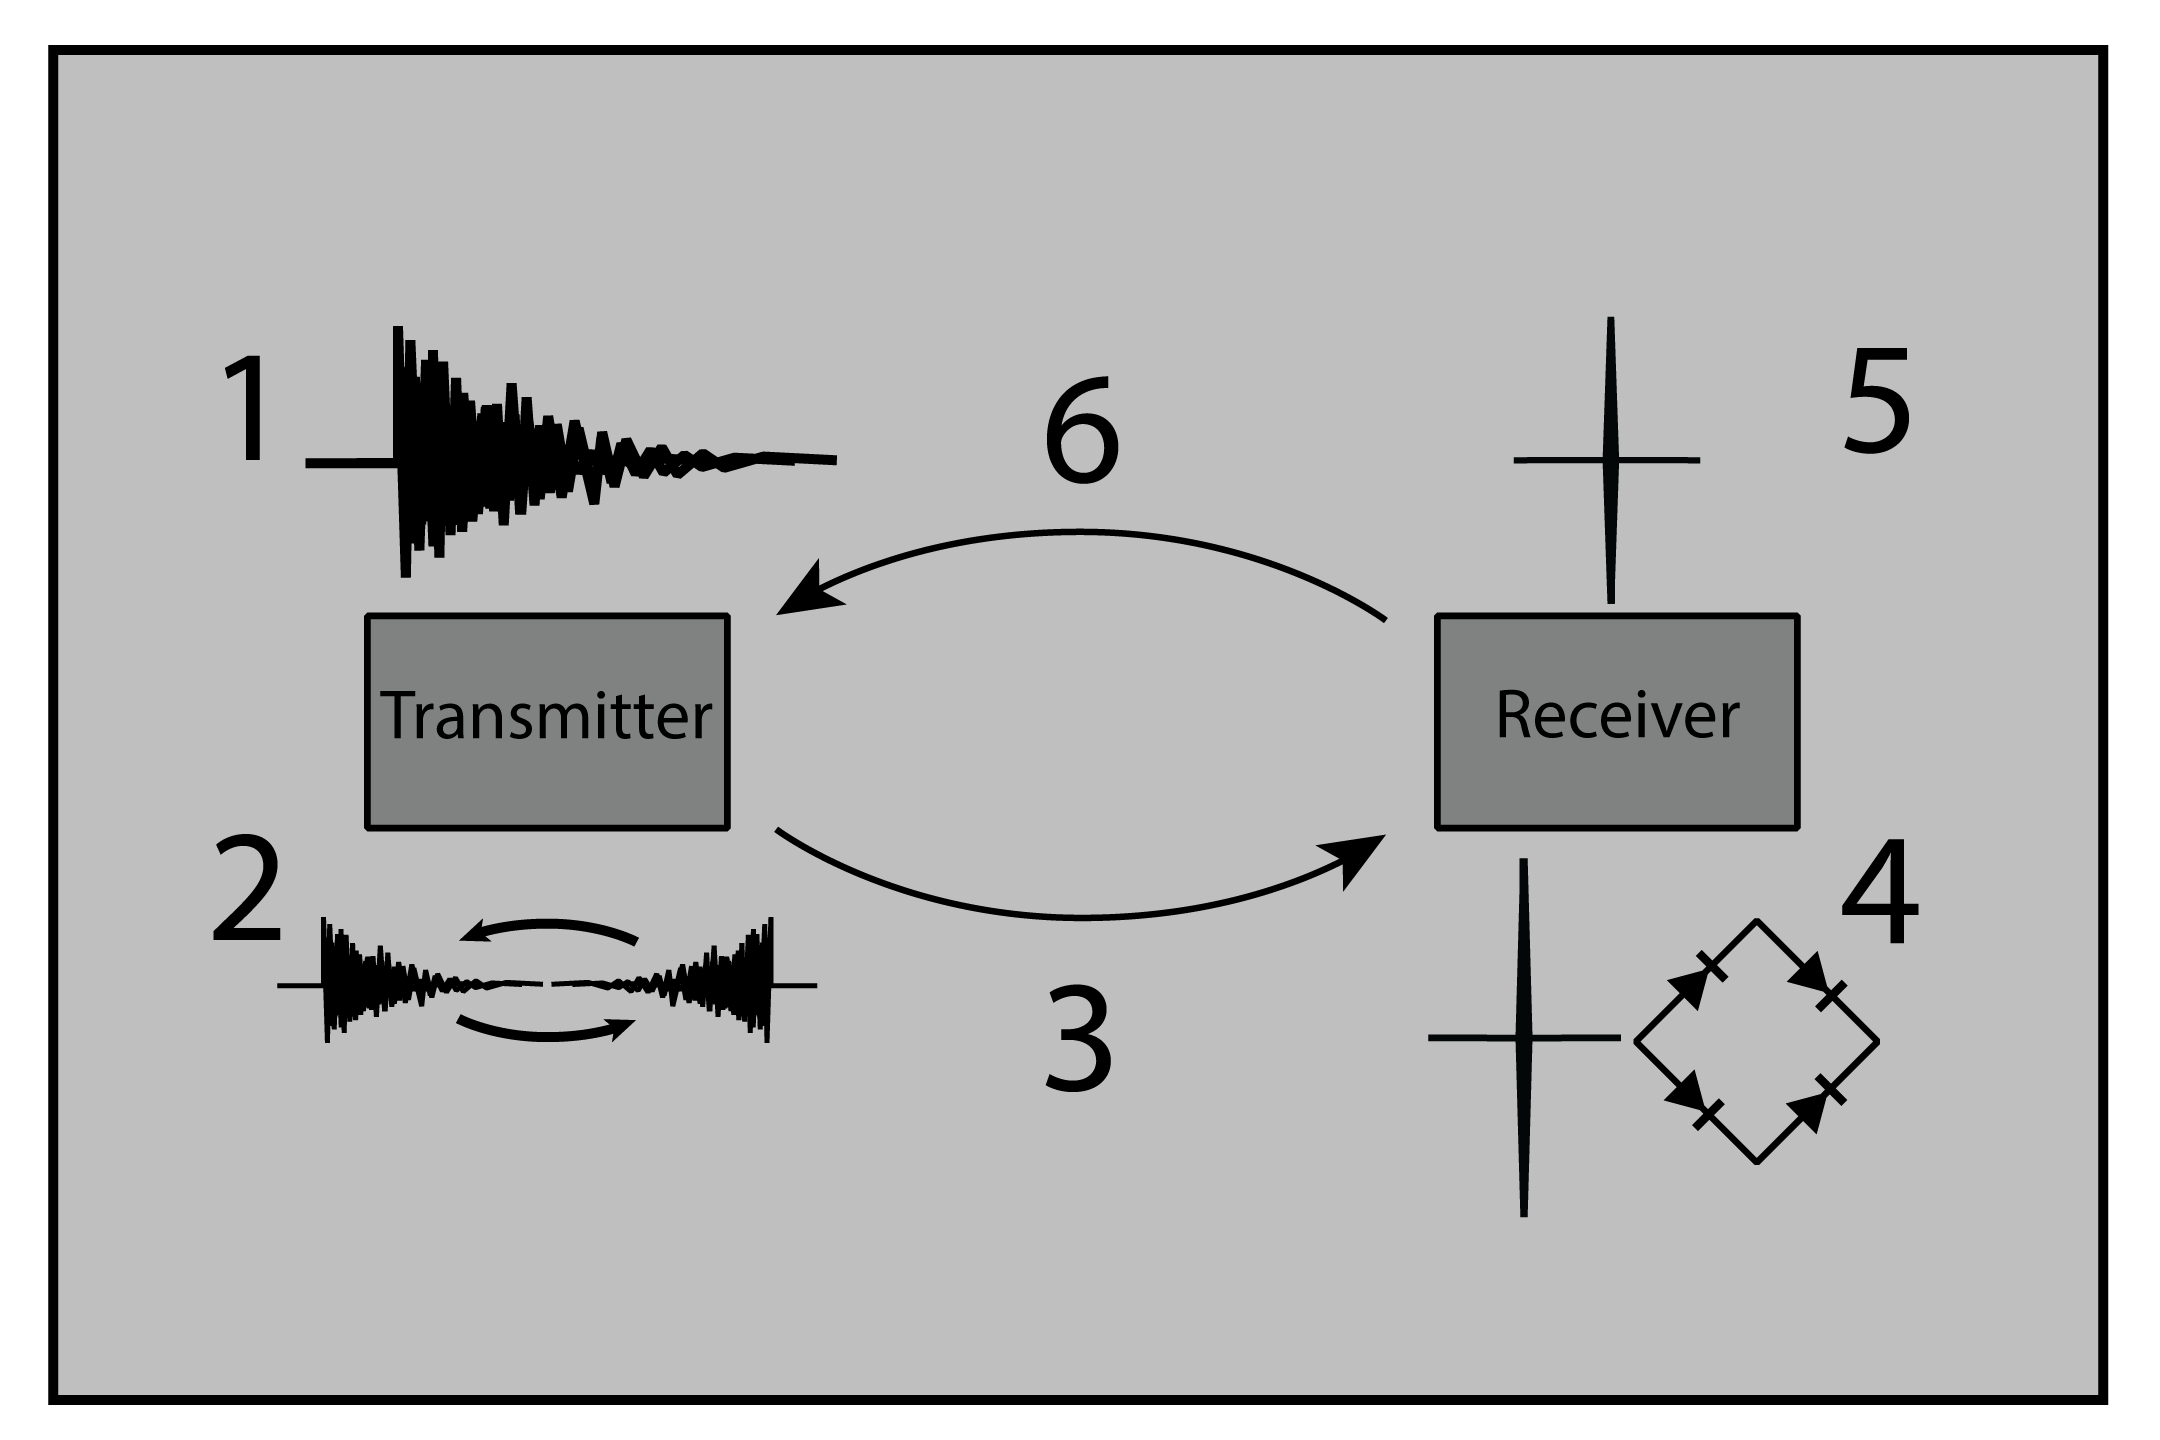
\includegraphics[width=\columnwidth]{figs/future/WPTSys}
\caption[Proposed Time Reversal System]{A notional time reversal WPT system. In the acquistion phase, a new receiver joins the system by broadcasting or emitting a characteristic signal (0). Here, the receiver actively emits a signal, but it is also possible for the transmitter to find a passive target, as shown in~\cite{nltr-wave-chaotic}. In either case, the next sona that the transmitter collects will contain spatial information unique to the receiver's location (1). In the power transfer cycle, the sona is time reversed (2), amplified, and broadcast back into the environment. The amplified signal reconstructs on the receiver (3) and is converted to usable DC power by the rectifier (4). A small fraction of the signal is used to re-broadcast a new characteristic signal (5) into the environment, which will be collected in the next sona (6). The cycle repeats from (2).}
\label{fig:SysImage}
\end{figure}

We have demonstrated the underlying concepts of the WPT system depicted in Figure~\ref{fig:SysImage}.
However, much work is necessary to transform this proof-of-concept technology to a functional product that consumers may use.
Future work discussed here falls into one of two categories. The first category includes established TR techniques that may be extended into the field of TR WPT.
The second category includes novel designs proposed by the team applicable only to TR WPT.

\section{Furthering the Understanding of TR WPT}
\label{sec:future-tr}
Imaging of objects and non-invasive surgery are already common applications of TR.
As a result, many techniques have been developed to improve reconstruction quality on a target.
We suspect that many of these techniques may have applicability to our proposed system, but did not
have the opportunity to investigate them in our research.

However, there are unique aspects of a TR WPT system that create avenues for research and innovation. Many of these deal with addressing the differing unique operating principles a TR WPT system. Most TR applications care little about operational environment, focusing only on the direct link between transmitter and receiver. TR WPT on the other hand is based off of a very paricular relationship between the transmitter, receiver, and the environment. Additionally, most TR applications consider stationary - or near stationary - targets. A practical TR WPT system must always consider moving targets, or at least stationary targets within a dynamic environment.

Some challenges in developing TR WPT may be addressed using modifications of techniques developed for other TR applications. We suggest that future research investigate the applicability of techniques such as iterative time reversal and exponential amplification to a practical WPT scheme. Other considerations set TR WPT apart from other TR research, and require the development of novel techniques. Below we suggest several experiments that could explore our knowledge of TR, and how the results of these experiments can benefit TR WPT.

\subsection{Iterations}

It has been well proven in the literature that time reversal focusing on an object can be repeated to improve waveform collapse on a target.~\cite{prada_iterative_1991} However, this technique has not yet been applied to TR WPT.

We suspect that applying iterative TR to reduce the effect of reflection orbits which contribute poorly to the final reconstruction, in favor of ones that do. The side lobes in the time domain are representative of energy that may not be able to be rectified unless they are combined into the main peak. We predict that we can maximize our efficiency and reconstruction quality using this method. Additionally, we predict that this method will only be useful for stationary targets. Because iterating the time reversal process takes several more steps, the length of time required to focus on a target is increased considerably. Since the technique for focusing upon a moving receiver proposed earlier relies upon repeating the time reversal process many times, it may not be acceptable for the time required to perform TR to increase several hundred percent.

Both of these characteristics can be easily tested, using algorithms already applied to acoustic TR. An experimental setup very similar to ours could be applied to this research. A faster sona refresh rate would be required from the TR system for this method to be able to outpace the natural ``decay'' of the testing environment. Once an iterative algorithm has been tested and found successful it should be tested in a less homogeneously reflective environment, to determine if it can be used to improve efficiency in lossy environments.

The novelty of such research is primarily in the characteristics measured. The demonstration (or lack thereof) of filtering of lossy paths would also be a major finding. Models should be generated relating the sona refresh rate to performance gains using iterative method. If possible, multiple environments should be tested to generalize these results.

\subsection{Multiple Transmitters}

All of the work in this thesis was conducted using a single transmitting antenna. The incorporation of multiple antennas would haved required major modifications to our experimental setup, and thus was beyond the scope of our study. However, previous work in time reversal in other fields, such as acoustics, have demonstrated the ability to improve signal quality through the use of multiple transmitters.

In one study, Mathias Fink demonstrated that a single-channel time reversal mirror acts like a spatiotemporal matched filter, where the time reveresal process is a convolution of the injected signal with a time reversed ``image'' of that signal. Using a 96-element antenna array, Fink showed that using multiple channels created a stronger collapse at the reconstruction time and that it tended to cancel the contributions of the temporal side-lobes, ultimately providing a better peak-to-noise ratio. When the number of channels is sufficient, the result is an inverse filter, which should produce the ideal reconstruction~\cite{fink-multi-channel}.

Although a practical wireless power transfer system will likely not be able to reach this theoretical limit, the positive relationship between number of elements and reconstruction strength should hold: namely, that adding $N$ elements to the time reversal mirror should increase the reconstruction strength by \textit{at least} a factor of $N$. In addition, it should reduce the accidental creation of ``hot spots'' at locations other than the intended reconstruction point, which would be a necessary safety concern to address in a practical system.

\subsection{Exponential Amplification}

Exponential amplification can be used to counteract decreased reconstruction quality caused by system losses~\cite{bini-thesis}. Exponential sona amplification is a nonlinear amplification to the sona across its timespan. It is meant to counteract the larger losses (due to larger number of reflections) experienced by reflective orbits with larger paths.

However, it should be understood that this method only compensates for the losses experienced by a time reversed signal. It does not avoid losses altogether, and in fact more energy is lost through this method. As a result, efficiency using this method should decrease. This introduces a tradeoff to using the method that could be significant to designers of a TR WPT system. It would be useful to quantify the effects of this tradeoff in a WPT context so that informed decisions can be made in the design of future systems.

\subsection{Sub Cavity}

The demand for optimal efficiency requires TR WPT to consider the characteristics of the environment moreso than ordinary TR applications. It is clear to the team that a TR WPT system will likely need some environmental modifications to achieve an efficiency sufficient to see practical application. These modifications should also be designed to be as cheap and simple to install as possible, to ensure that system price remains practical.

We suggest a method of improving efficiency of TR wireless power transfer by introducing a ``sub cavity'' within the transfer environment. This ``sub cavity'' will be defined as a region of the environment that allows extremely efficient TR WPT. The sub cavity becomes much less lossy than the environment as a whole. TR paths will preferentially move through the sub cavity, and can dramatically improve the efficiency of the entire system. A successful sub cavity must have the following characteristics:

\begin{itemize}
  \item High transfer efficiency/low reflective losses
  \item Chaotic geometry to facilitate the function of TR
  \item Presence of one or more paths between the sub cavity and main environment
\end{itemize}

There are many methods that could potentially generate such a cavity - a proposal for such as system can be found in Figure~\ref{fig:subCav}. This cavity is a thin sheet of material that would be mounted to the ceiling of the room in question. The material in this sheet should have a smaller index of refraction than air; as a result any signal broadcast into can become ``trapped'' in the layer. At any given point along the barrier of the sub cavity only small amounts of signal will return to the main environment. A TR WPT system can selectively choose paths through the sub cavity that will focus on a given receiver with high transfer efficiency. Reflectors can be added to the sub cavity as needed to ensure that its complexity is enough to allow TR to occur.

\begin{figure}[h]
\centering
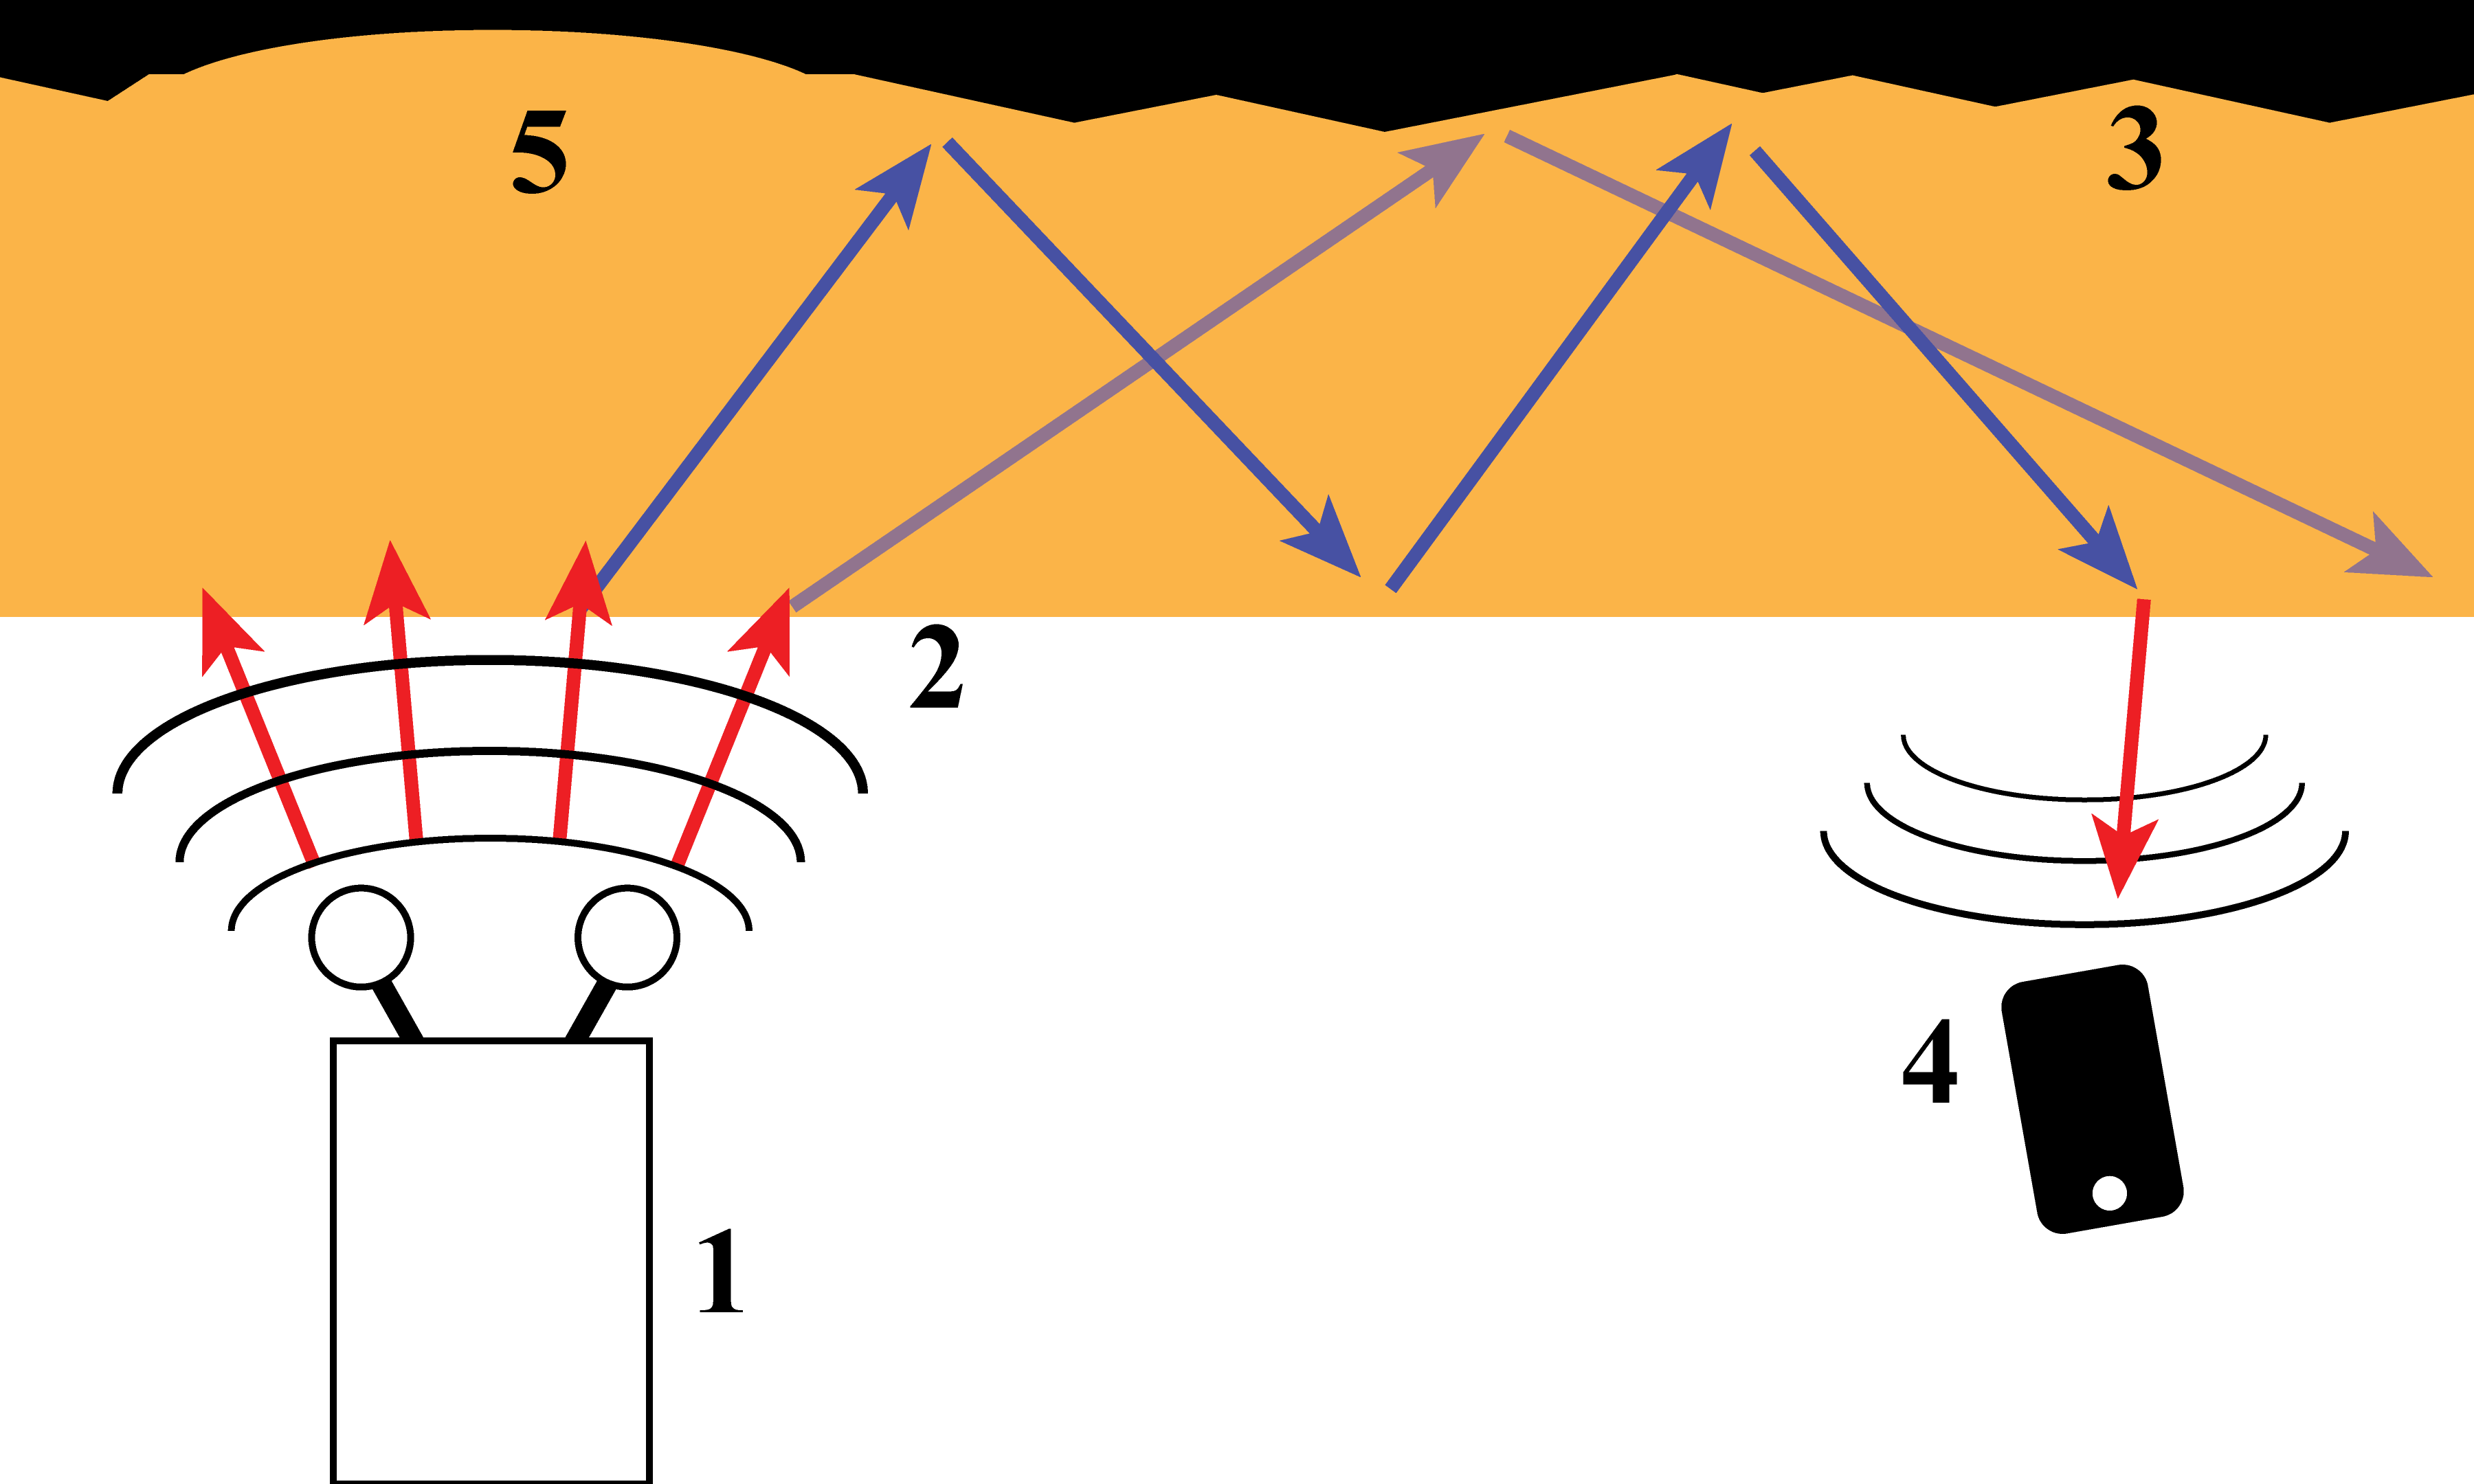
\includegraphics[width=\columnwidth]{future/subCavity}
\caption[Proposed ``Sub Cavity Design'']{A proposed sub cavity design. A transmitter (1) broadcasts an interrogation pulse into the environment. When the pulse reaches the low index of refraction material of the sub cavity, it refracts, taking on a lower angle (2). The interrogation pulse totally internally reflects within the cavity (3), until returning to the main environment. Some aspects of the signal reach the receiver, allowing a TR link to be established (4). A focal aspect of the geometry above the transmitter (5) is highlighted as a way of improving transmission.}
\label{fig:subCav}
\end{figure}

Research would focus on, firstly, proving that this method can work for the purposes of increasing efficiency of transfer. Once this has been established, the geometry of the sub cavity should be optimized to work in a wide range of potential environments. Uniformity of signal coverage is a major concern, and must be tested either experimentally, or through use of simulation software.
